\section{Modal truncation}
\subsection{Diagonal Canonical Form} \label{dcnf}
A LTI system \((A, B, C, D)\) with transfer function \(G(s)\) can be written in the following way:
\begin{gather}
I = \{1, 2, \hdots, n\} \\
G(s) = D + \sum_{i \in I} \frac{\Phi_i}{s-\lambda_i} \label{dcnf}
\end{gather}

The set \(\Lambda = \{\lambda_1, \hdots, \lambda_n\}\) denotes the eigenvalues of the matrix \(A\) in state space.
This resembles the partial fraction decomposition of \(G(s)\) \cite{vuillemin2020optimal}.
The residue \(\Phi\) can be computed using the eigendecomposition of \(A\) and using the eigenvectors for a coordinate transform:
\begin{gather}
AX = X\Delta \quad X \zeta =  x 
\end{gather}
The system matrices have to be transformed accordingly:
\begin{gather}
\hat{A} = X^{-1}AX = \Delta \\
\hat{B} = X^{-1}B \quad \hat{C} = CX \\
\hat{D} = D
\end{gather}
Those transformed matrices are used to calculate the transfer function \ref{tf-from-ss}:
\begin{gather}
G(s) = CX(sI - \Delta)^{-1}X^{-1}B + D\\
= D + \begin{bmatrix}
C x_1 && \hdots && Cx_n
\end{bmatrix} diag\{\frac{1}{s-\lambda_1}, \hdots, \frac{1}{s-\lambda_n}\} \begin{bmatrix}
x_1^{-1}B \\
\vdots \\
x_n^{-1}B
\end{bmatrix} \\
= D + \sum_{i \in I} \frac{c_i b_i^{T}}{s - \lambda_i} 
\Rightarrow \Phi_i = c_i b_i^{T}
\end{gather}
\cite{Benner}

\subsection{Optimal Modal Truncation}
The goal of modal truncation is to find a subset of the indices \(I\)  such that only \(r\) elements are contained in this subset:
\begin{gather}
I_r \subseteq I, \quad |I_r| = r
\end{gather}
Using this subset as indices in \ref{dcnf} a truncation is obtained, yielding a system defined by a new transfer function \(\hat{G}(s)\).
The set \(I_r\) has to be chosen such that the error \(||G(s) - \hat{G(s)}||_{H_n}\) becomes minimal.
Here  \(H_n\) denotes the \(H_2\)  norm.
As shown in \cite{vuillemin2020optimal} other norms are also usable but for simplicity only the stated norm is used.
Furthermore in case some \(\lambda_i \in \Lambda, Im(\lambda_i) > 0\) is a complex number  \(i \in I_r\), the index of the according complex conjugate eigenvalue has to selected too, if \(\lambda_j = \bar{\lambda}_i \in \Lambda \wedge i \in I_r \Rightarrow j \in I_r\). 
This yields the following optimization problem:
\begin{gather}
G_{\alpha}(s) = D_{\alpha} + \sum_{i \in I} \alpha_i \frac{\Phi_i}{s - \lambda_i} \\ 
\min_{\alpha} ||G(s) - G_{\alpha}(s)|| \\\ s.t. \quad
\alpha^{T}\alpha = r \\
J = \{(\lambda_i, \lambda_j) \in I | \lambda_i \in \mathbb{C}, Im(\lambda_i) > 0, \lambda_i = \bar{\lambda_j}\} \\
a_{.,j} = -a_{.,l} = 1, \quad	(i, j) \in J \\
A\alpha = 0
\end{gather}
Where \(\alpha \in \{0, 1\}^{n}\) is some binary vector with \(\alpha^{T} \alpha = r\) that represents the selection of indices.
By defining the error of that system as:
\begin{gather}
\epsilon_{\alpha}(s) = G(s) - G_{\alpha} \\
||\epsilon_{\alpha}(s)||_2^2 = \sum_{i, k \in I} (1-\alpha_i) \frac{tr(\phi_i \phi_k^{T})}{-\lambda_i - \lambda_k}(1-\alpha_k) \\
||\epsilon_{\alpha}(s)||_2^2 = (1-\alpha)Q(1-\alpha) \\
q_{ij} = \frac{tr(\phi_i \phi_k^{T})}{-\lambda_i - \lambda_k^*}
\end{gather} 
This leads to a new optimization problem:
\begin{gather}
\min_{\alpha} \quad (1-\alpha)Q(1-\alpha) \label{opt-h2}\\
s.t. \quad \alpha^T\alpha = r \\
A\alpha = 0
\end{gather}
\cite{vuillemin2020optimal}
\subsection{Applying Modal Truncation to Heat Equation} \label{mtht}
As described in \ref{heat-ss} the system matrices \((A, B, C, D)\) can be obtained for the given heat equation.
Now by applying \ref{tf-from-ss} yields the corresponding transfer function \(G(s)\).
By calculating the partial fraction decomposition as described in \ref{dcnf} the DCNF can be obtained.
Since \(B\) and \(C\) are given by some identity matrix and \(D\) is a zero matrix the upper error bound of the error in \(H_2\) norm is given as
\begin{gather}
||\epsilon(s)||_{H_2} \leq \sum_{i \in I_r^{c}} \frac{1}{\sqrt{-2Re(\lambda_i)}}
\end{gather}\cite{vuillemin2020optimal}. 
Since for stable systems \(Re(\lambda) < 0 \forall \lambda \in \Lambda\) this upper bound can be expressed as follows with \(\Lambda_{\epsilon} = \{Re(\lambda_i)| \lambda_i \in \Lambda i \in I_r^{c}\}\)
\begin{gather}
||\epsilon(s)||_{H_2} \leq \sum_{i \in I_r^{c}} \frac{1}{\sqrt{2|Re(\lambda_i)|}} \leq \frac{|I_r^{c}|}{\sqrt{2|\max(\Lambda_{\epsilon})|}} \\
\end{gather}
To minimize this upper bound \(|\max(\Lambda_{\epsilon})|\) has to be maximized.
This is achieved by selecting the entries of \(\Lambda_{\epsilon}\) such that it contains \(n - r\) largest real parts of the eigenvalues in \(\Lambda\).

Figure \ref{FIG-MT} shows a solution to heat equation using FEM and an approximation using MT with \(u(x, t) = 0, x_0 = 10000^{70\times1}, n = 70, n_{approx} = 10\).
\begin{figure}[H]
\centering
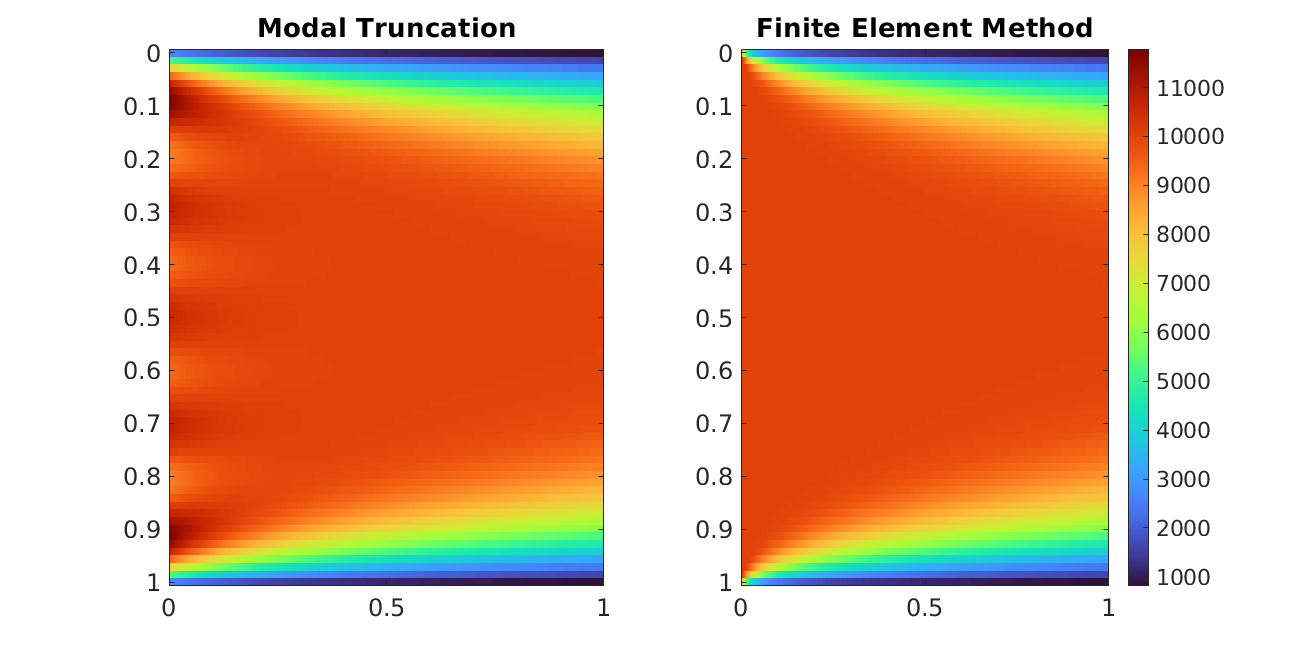
\includegraphics[ width=12.5cm]{images/mt}
\caption{FEM solution and MT approximation for heat equation}
\label{FIG-MT}
\end{figure}

